\documentclass[preprint]{elsarticle}




\usepackage[ruled]{algorithm2e}
\usepackage{algpseudocode}
%\usepackage{algorithm}
%\usepackage{algorithmic}
\usepackage{graphicx}
\usepackage{epstopdf}
\usepackage{url}\renewcommand{\baselinestretch}{1}
\usepackage{epsfig}
\usepackage{amsmath,amssymb}
\usepackage{multirow}
\usepackage{caption}
\usepackage{fancyvrb}
\usepackage{mathptmx}
\usepackage{alltt}
\usepackage{amsmath}
\usepackage{comment}
\usepackage{amsfonts}
%\usepackage[switch, modulo]{lineno}
%\usepackage{algpseudocode}
\usepackage{booktabs}
%\usepackage{tikz}
\usepackage{tabularx}
\usepackage{float}
\usepackage{array}
\usepackage{subcaption}
\usepackage[english]{babel}
%\newcolumntype{L}{>{\centering\arraybackslash}m{3cm}}
%\usepackage{lineno,hyperref}
\usepackage{amsthm}
\usepackage{lipsum,amsmath,multicol}
\usepackage{enumitem}
\usepackage{slashbox,pict2e}
\usepackage{array}
\usepackage{bbm}
\usepackage[normalem]{ulem}
\usepackage{wrapfig}
\newtheorem{theorem}{Theorem}
\setcounter{theorem}{0}
\theoremstyle{definition}
\newtheorem{definition}{Definition}
\setcounter{definition}{0}
\theoremstyle{remark}
\newtheorem{remark}{Remark}
\newtheorem{lemma}[theorem]{Lemma}
\newtheorem*{cor}{Corollary}
\theoremstyle{property}
\newtheorem{property}{Property}
\setcounter{property}{0}
\newtheorem{condition}{C}
\setcounter{condition}{0}
\newtheorem{conditions}{Condition}
\setcounter{conditions}{0}
%\newtheorem{property}[theorem]{Property}

\begin{document}

\title{On Trustworthy Federated Clouds: A Coalitional
Game Approach}

\author{Adel Abusitta, Martine Bellaiche$\tnoteref{t2}$, and Michel Dagenais\\
Department of Computer and Software Engineering,\\ Ecole Polytechnique de Montr´eal, Montr´eal, Canada\\
Email:\{adel.abusitta,martine.bellaiche,michel.dagenais\}@polymtl.ca}
\tnotetext[t2]{Corresponding Author}

\begin{abstract}
The demands for cloud-based applications are expected to increase in such a way that current Cloud Providers' (CPs) resources may become insufficient. This promotes the need to outsource some of the requested Virtual Machines (VMs) to other CPs. A Cloud Federation (CF) provides an effective platform that enables CPs to upgrade their resource scaling strategies. Several CF approaches have been proposed, but they suffer from the hazard of working with untrusted (malicious or not) CPs, resulting in performance degradation. To address this problem, we introduce a trust-based framework for CF formation. Our model enables a CP to evaluate other CPs' trustworthiness by considering two
approaches: objective and subjective trust evaluations. In the former, Bayesian inference is used to compute trust values based on previous interactions. In the latter, the Dempster-Shafer Theory (DST) is used to compute trust values in the absence of previous interactions. Thereafter, a federation formation algorithm is devised, based on coalitional game theory, that allows CPs to cooperatively establish their federations in such a way that maximises the trust of the formed federations. Experimental results show that our proposed algorithm enhances throughput, response time and availability of federated CPs compared to the QoS-based and grand formation models.

\end{abstract}

% Note that keywords are not normally used for peerreview papers.
\begin{keyword}
Cloud federation; trust; virtual machines; game theory
\end{keyword}


% make the title area
\maketitle


% To allow for easy dual compilation without having to reenter the
% abstract/keywords data, the \IEEEtitleabstractindextext text will
% not be used in maketitle, but will appear (i.e., to be "transported")
% here as \IEEEdisplaynontitleabstractindextext when compsoc mode
% is not selected <OR> if conference mode is selected - because compsoc
% conference papers position the abstract like regular (non-compsoc)
% papers do!

% \IEEEdisplaynontitleabstractindextext has no effect when using
% compsoc under a non-conference mode.


% For peer review papers, you can put extra information on the cover
% page as needed:
% \ifCLASSOPTIONpeerreview
% \begin{center} \bfseries EDICS Category: 3-BBND \end{center}
% \fi
%
% For peerreview papers, this IEEEtran command inserts a page break and
% creates the second title. It will be ignored for other modes.


\section{Introduction}
\label{Sec:Intro}

Cloud Computing enables Cloud Providers (CPs) to rent out space on their infrastructures, platforms and services to many consumers. This becomes possible thanks to virtualization that enables the easy migration of applications and services from one node to another. Many companies, organizations and
governments are expected to transfer, if they have not already, all or parts of their IT solutions to the cloud \cite{gonzales2015cloud}. This transfer is profitable from an economic point of view since it allows them to streamline technology infrastructure expenses and capital costs.

One of the main issues that must be faced by CPs, due to the huge demands on their services, is the problem of insufficient resources to fulfill
the requested VMs. This promotes the need for CPs
to delegate these requests to other CPs in order
to upgrade their resource scaling capabilities. A Cloud Federation (CF) provides an effective platform to address
the aforementioned challenges \cite{rochwerger2011reservoir}. The purpose of the CF
consists of grouping CPs to fulfill the dynamic
resource requests of users/applications to support data-intensive
workloads \cite{celesti2010enhance}. Thus, through the use of CFs, CPs can benefit from each other's
resources to run the VMs \cite{guazzone2014game} \cite{rochwerger2011reservoir} \cite{celesti2010enhance}, in order to improve individual performance and enhance users’ satisfaction.

Existing works in CF (e.g. \cite{buyya2010intercloud} \cite{celesti2010enhance} \cite{fazio2015enhance} \cite{goiri2010characterizing} \cite{mashayekhy2015cloud}) significantly focus on forming the federation among CPs by considering those that provide high
availability, profits and QoS. Although the orientation of these approaches is promising and may contribute to enhance CPs' performance, these approaches often suffer from the hazard of choosing unreliable CPs in the federation, resulting in performance degradation and loss of CPs’
reputation due to Service Level Agreement (SLA) violations between the users and the federation.

\textit{Example.} Consider a CP that does not have
sufficient resources to fulfill the requested VMs, and
needs to outsource some of the requested VMs to other
providers within the federation. If the trust issue is
not considered during the federation formation, there will be several reasons that make delegated CPs unable to achieve requests as expected. These reasons include the following: inadequate maintenance causing frequent breakdowns, poor security causing compromised nodes or nodes slowed down by a DDoS (Distributed Denial-of-Service Attack) and lack of capacity
for the load accepted. Also, the delegated CP might be selfish and/or malicious and refuse to share enough resources. Worse, it may even drop the requests.
Such unreliable delegated CPs result in performance degradation, decreased revenues and poor users’ satisfaction as well as Service Level Agreement (SLA) violations. Indeed, ‘’trust’’ has different meanings in various disciplines (e.g. psychology, politics, economy). In this paper, trust is interpreted as the degree of the belief that a delegated CP in a given federation will achieve its tasks as it should \cite{bu2011distributed} \cite{hassan2015qos}.

To address the aforementioned problems, we propose a flexible trust-based framework for federation formation. Our framework can be summarized
as follows. We let CPs evaluate a trust value for each other by adopting two approaches: objective and subjective trust evaluations. In the former, the trust value is computed from direct observation. The CP's trust value is evaluated based on its previous interactions (i.e. experience) using Bayesian inference. In the latter, the Dempster-Shafer Theory (DST) of evidence is used when there is no previous interactions among CPs. Thereafter, we propose a federation formation algorithm that is based on the coalitional game theory \cite{ray2007game}. The algorithm enables CPs to leave or join a given federation in such a way that enhances their trust among CPs.

Unlike similar works (e.g. \cite{hassan2015qos}), we adopt a distributed
mechanism in which each CP autonomously makes its own decisions. This, in turn, avoids the difficulty of finding a trusted third party. Also, it reduces instability inside the federation due to single point of failure. In summary, our work consists of the following contributions:

\begin{itemize}

\item Modeling and proposing a decentralized framework that considers the trustworthiness of heterogeneous CPs during
the formation of cloud computing federations. More specifically, we present a systematic approach that associates the
trustworthiness of CPs through the formation procedure.

\item Proposing a new trust evaluation approach, based on Bayesian inference, that enables a CP to evaluate another CP's trustworthiness based on their previous interactions and experiences.

\item Proposing a new trust aggregation technique, based
on the Dempster-Shafer Theory (DST) \cite{shafer1992dempster}, that enables a CP to derive a trust value in cases where there were no previous interactions and experiences.

\item Devising a federation formation algorithm, based on a coalitional game theory, that allows a set of CPs
to cooperatively build their federations in such a way that maximises federations trust. The proposed algorithm converges to a Nash-stable situation; that is, no CP has an incentive to leave its current federation to move to
another federation.
\end{itemize}


%\cite{wahab2015misbehavior}

The remainder of the paper is organized as follows. In Section 2, we discuss the related work. We present the trust model and assumptions in Section 3. In Section 4, we present the proposed federation formation framework. In Section 5, we present our empirical results. Finally, Section 6 concludes the paper.


\section{Related Work}

The concept of federations among CPs was first introduced
by Rochwerger et al. \cite{rochwerger2011reservoir}. Although their work
shows the main materials needed to achieve federation, they
did not show the architectural elements that compose multi-cloud
computing environments. Buyya et al. \cite{buyya2010intercloud} introduce the
challenges and architectural elements for federations. Similarly,
Celesti et al. \cite{celesti2010enhance} and Fazio et al. \cite{fazio2015enhance} present a cloud architecture
that allows CPs to build a federation with each other. They consider two kinds of CPs: home
and foreign. The home CPs are those that
are unable to fulfill the consumers' tasks and therefore
forward these jobs to the foreign CPs. Similarly, Goiri et al. \cite{goiri2010characterizing} present
a decision-based model that helps a CP
decide on forming federations with public CPs in
order to maximize their individual profit.

Toosi et al. \cite{toosi2011resource} present multi-resource provisioning
policies, that assist the CPs to increase their resource
utilization and profit. Their model can terminate VMs whenever the profit of shutting them down exceeds
the profit of running such VMs. Also, Van den Bossche et
al. \cite{van2010cost} present a binary integer program model that
minimizes the cost of outsourcing, using a mix of public
and private providers. Chaisiri et al. \cite{chaisiri2012optimization} propose an
optimal VM provisioning algorithm using stochastic programming
that considers multi-cloud providers with the
objective of maximizing their profit. Similarly, Bruneo
\cite{bruneo2014stochastic} proposes a performance evaluation approach based on
stochastic reward nets for federated CP. The model
predicts and quantifies the cost-benefit of a strategy portfolio
and the corresponding QoS experienced by clients.

A business-oriented cloud federation model for real-time applications is proposed by Xiaoyu
et al. \cite{yang2012business}. The model allows multiple heterogeneous CPs to cooperate and provide
scalable infrastructure. The advantage is the business layer added to
support the federations. The layer can trigger on-demand resource provisioning across
multiple CPs and therefore helps maximize the clients satisfaction and business benefits \cite{yang2012business}.

Salama \& Shawish \cite{salama2014qos} present a QoS-based approach for cloud federation. They use QoS metrics
such as throughput and response time during the federation formation process. By considering QoS metrics, the federation helps eliminate Service Level Agreement (SLA) violations and maximise QoS targets.
In \cite{mashayekhy2015cloud}, Mashayekhy et al. propose a hedonic coalitional
game to achieve cooperation among IaaS services.
Based on the federation coalition game, they design a
cloud federation formation mechanism that allows
CPs to form federations that maximize their
profits.

A game theoretic approach for cloud federation is
also proposed by Hassan et al. \cite{hassan2011distributed}. The study enables
the dynamic resource allocation in a cloud federation. They
define a price function for a CP that gives incentives to
other CPs to contribute their resources in order to form
a federation. Similarly, Mihailescu \& Teo
\cite{mihailescu2010dynamic} present a strategy-proof dynamic pricing scheme for
cloud federations. In \cite{li2013profit}, Li et al. propose profit maximization
strategies in cloud federations. They present a
truthful auction-based mechanism for selling VMs within a federation. This enables cloud federation members to sell
or buy resources in a way that maximises their profit.
Also, Samaan \cite{samaan2014novel} proposes an economic model for
sharing resources among CPs in the federation.

Few studies have addressed trust issues in cloud federations. For example, Ngo et al. \cite{ngo2012toward} present an approach for attribute-based trust establishment to be used in the multi-cloud environment. They propose an approach for trust evaluation and delegation. Messina et al. [24] suggest a trust model based on the reputation. The model allows users to properly select a suitable CP on the basis of reliability and reputation. In \cite{wahab2016towards}, Abdel Wahab et. al. propose a trust-based federation formation model to be among functionally-similar cloud's services, where these services and applications should work as one entity, called community. The main limitation of this approach is that it works only with homogeneous environment for formatting communities. Similarly, Hassan et al. \cite{hassan2015qos} propose a trust-based cloud federation formation mechanism based on the cooperative game theory. The mechanism allow CPs to dynamically join a federation based on maximization of profits and minimization of penalty costs. The main limitation of this approach is that it is based on a centralized
architecture, whereby a trusted third-party called broker \cite{medjahed2005dynamic} is responsible for formatting the federation.

Overall, for a multi-cloud environment, a decentralized framework that considers trustworthiness of heterogeneous CPs during the forming of federations has yet to be addressed. Thus, in this paper, we present a systematic schema that considers the trustworthiness of CPs through
the cloud federation formation process. This enhances CP's performance, revenues and clients’ satisfaction.

\section{Trust Model and Assumptions}

In this section, the definition and properties of trust in the context of cloud federations are explained. Based on the definition, the trust model used to formulate trust among CPs in the federation is described. Furthermore, our methodology is also introduced. Table 1 summarizes the different notations that are used in this section.

\begin{table}[!ht]
\caption{Notations}
\centering
\begin{tabular}{|c c|}
\hline
Symbol & Significance \\
\hline
$F$ & Federation \\
$F_{k}$ & Federation $k$\\
$\mathcal{N}$ & set of CPs \\
$N$ & Number of CPs \\
$\Pi$ & Set of federation partitions \\
$T_{i}^{j}$ & The trust value of CP $j$ with respect to the CP $i$.  \\
$U_{i}(F_{k})$ & i's federation trust criterion of a given federation $k$ \\
\hline
\end{tabular}
\end{table}

\subsection{Definition of Trust}
Trust can take on different meanings in different disciplines (e.g. psychology, politics, economy). In this paper, we define trust as a degree of belief that a CP, in a given federation, will achieve its tasks as expected. Based on this definition, untrusted CP are not necessary malicious. A malicious CP may accept to share other CPs with the intention of dropping other CPs’ jobs and refuse to share its resources within the federation. Moreover, the CP may not be malicious yet still deficient. For example, inadequate maintenance causing frequent breakdowns, poor security causing compromised nodes or nodes slowed down by DDoS and lack of capacity for the load accepted. All of these scenarios may affect achieving tasks as expected.

\subsection{Trust Model}
The aforementioned definition is used to establish our trust model.
We evaluate trust in the proposed scheme using a real number
$T$ with a continuous value between 0 and 1. In our model, trust is made up of two components: direct and indirect observations. In direct observation trust,
an observer estimates the trust of a CP based
on its own experience. Thus, the trust value consists of the anticipation
of a objective probability used by a CP to decide whether
another CP is reliable or not. A trust value from direct observation is computed using Bayesian inference. This process is explained in detail in Section 4.1.

The use of direct observations requires that a trustor has had previous interactions with a CP in order to give its judgement and derive a trust value. If we only consider direct observations, evaluating the trust value of a new CP (i.e. a cloud without any previous interactions) becomes impossible. We tackle this problem by considering another way of obtaining trust. This is done by collecting judgments on this CP from other CPs that previously interacted with that CP. Therefore, the trust value becomes the anticipation of a subjective probability used by a CP to decide whether
another CP is reliable or not. The Dempster-Shafer Theory (DST) \cite{yu2002evidential} is an adequate candidate to support this situation, in which evidences are collected from CPs that may be unreliable. A detailed explanation of this process is included in Section 4.2.

Based on the obtained trust values, a trust-based federation formation algorithm is presented. The algorithm is based on the coalitional game theory \cite{ray2007game}, \cite{dreze1980hedonic}, \cite{apt2009generic}, where each coalition represents a given federation $F$.

Given the set $\mathcal{N}$ = $\{$1, 2, . . .,N $\}$ of CPs, a federation $F \subseteq \mathcal{N}$ represents an
agreement among the CPs in $F$ to delegate tasks among each other. Let $\Pi = \{F_{1}, . .. , F_{l}\}$ represent the set of federation partitions. That is, for $k$ = $\{$1, 2, . . . , l$\}$, each $F_{k}$ $\subseteq$ $\mathcal{N}$ is a disjoint federation. The algorithm enables each CP $i$ $\in$ $\mathcal{N}$ to decide whether to join a given federation $F_{k} \in \Pi$ or not based on the federation trust criterion calculated by CP $i$. Each CP $i$ determines the federation trust criterion $U_{i}(F_{k})$ of any given federation $F_{k} \in \Pi$ by calculating the product of the trust values of all the CPs in that federation:

\begin{equation}
U_{i}(F_{k}) = \prod _{{j}\in F_{k}} T_{i}^{j}
\end{equation}

where $T_{i}^{j}$ denotes the trust value of CP $j$ with respect to the CP $i$.

The use of the product in the definition of the federation trust criterion instead of summation, is due to the fact that the former enables a very small CP trust value to have a significant impact on the result. Therefore, its impact will not be mitigated by a higher value as in the case of summation. A detailed explanation is included in Section 4.3.

Based on the above discussion, the methodology of the proposed scheme is shown in Figure 1.

\vspace{2mm}
\begin{figure*}[!ht]

\centering
\scalebox{0.55}{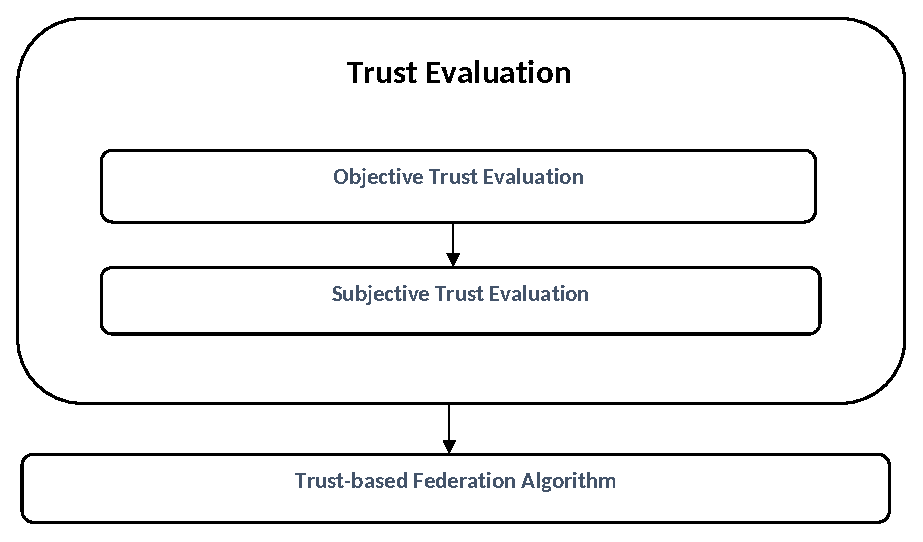
\includegraphics{framework.eps}}
\label{fig1}
\caption{Proposed Methodology}
\end{figure*}

\vspace{2mm}

\section{The Proposed Trust-based Federation Formation Framework}

In this section, a trust-based federation formation framework is presented. The section is divided into the following subsections: objective trust evaluation, subjective trust evaluation and trust-based federation formation algorithm.


\subsection{Objective Trust Evaluation: Direct Observation}

%\cite{desnoyers2006lttng}\cite{sivakumar2010effectiveness}
In this section, the proposed objective trust
evaluation approach is introduced. In this model, each CP calculates
the trust value of another CP based on its experience with that provider (i.e. direct observation). First, the methodology used to compute trust values is discussed. Then, trust bootstrapping issues are presented.

%\cite{desnoyers2006lttng}
%\cite{desnoyers2006lttng}
\subsubsection{Trust computation}
Based on what we presented earlier, a CP can directly evaluate the trust value of another CP based on their experience with that CP. We adopt
a Bayesian inference approach to compute the trust value of a CP \cite{josang2002beta}. The Bayesian inference was chosen because it is
well-founded to derive objective trust values \cite{yahyaoui2012trust}. The trust value can be promoted if the
cloud successfully performs a task as expected and it can be demoted otherwise. A CP $i$ $\in$ $\mathcal{N}$, is endowed with a belief function, which computes the trust level of another CP $j$ $\in$ $\mathcal{N}$, that previously collaborated with CP $i$. The
new trust value $t'_{j}$ is derived from the old trust value $t_{j}$ (we discuss later how to obtain the initial trust value) as follows:

\begin{equation}
t'_{j}=F(t_{j};\alpha_{j},\beta_{j})
\end{equation}

The incomplete beta function $F$ is the cumulative beta distribution function
of the Beta Probability Density (BPD) function, which is defined as follows:

\begin{equation}
f(x;\alpha_{j},\beta_{j})=\frac{x^{\alpha_{j}-1}(1-x)^{\beta_{j}-1}}{\mathbf{Beta}(\alpha_{j},\beta_{j})}
\end{equation}

The value of $\alpha_{j}$ and
$\beta_{j}$ are updated after the execution of each task
by the CP $j$. $\beta_{j}$ is increased when a CP $j$
performs a given task as expected. Eq. (4) describes the
update of $\beta_{j}$.

\begin{equation}
\beta_{j} = \beta_{j} \times (1+\mu_{j})
\end{equation}

where $\mu_{j}$ represents the weight of performing the task by
CP $j$ if it is successful and 0 if not.

Eq. (5) describes the update of $\alpha_{j}$.

\begin{equation}
\alpha_{j} = \alpha_{j} \times (1+\nu_{j})
\end{equation}

where $\nu_{j}$ denotes the weight of performing the task by the
cloud if it is unsuccessful and 0 if not.

The values of $\mu_{j}$ and $\nu_{j}$ should be carefully set by a CP $i$ who is allocating the jobs. These values reflect the importance of the tasks assigned to the delegated CP. Note that a higher value of $\beta_{j}$ will increase the trust of a CP $j$ while a higher value of $\alpha_{j}$ will decrease it.

The initial trust value $t_{j}$ is calculated at the beginning through the testing period. The total reported request task from  CP $j$ is denoted by the set $\mathcal{M}_{j}$. The initial trust value represents the total number of successfully performed tasks over the total number of tasks:

\begin{equation}
t_{j}=\frac{\sum_{k \in \mathcal{M}_{j}} r_{j,k}}{|\mathcal{M}_{j}|}
\end{equation}

Where the parameter $r_{j,k}$ is the revealed result of the k-th task request: $r_{j,k}$ =1 indicates successful perform of the k-th request. $r_{j,k}$ =0 indicates otherwise.

The initial value of $\alpha$ and $\beta$ can be obtained as follows:

\begin{equation}
\alpha_{j}=\sum_{k \in \mathcal{M}_{j}} (1 - r_{j,k})
\end{equation}

\begin{equation}
\beta_{j}=\sum_{k \in \mathcal{M}_{j}} (r_{j,k})
\end{equation}

\subsection{Subjective Trust Evaluation: Indirect Observation}
Computing the objective trust value of a CP requires some interactions to be established
between CPs. In other words, an experience with a certain CP is required in order to evaluate
its performance in achieving tasks. In some situations, evaluating the trust value of
a CP using that method cannot be achieved without interactions between
CPs. To address this problem, an DST-based aggregation technique is proposed [33].
DST is a mathematical theory that aggregates evidences from independent sources to
come up with a degree of belief regarding a certain hypothesis [33]. DST was selected
for the following main reasons: (1) unlike other aggregation approaches (e.g. Bayesian
approach) that demand complete knowledge of prior probabilities, DST can handle a
lack of complete knowledge (i.e. uncertainty), and (2) it has a property to prevent collusion
attacks, which occur when several malicious CPs collaborate to give misleading
judgments. This attack can be performed either to increase the trust value of some CPs
or to decrease the trust value of other CPs. Note that the DST is regarded as a useful
approach in uncertain reasoning and is widely used in distributed multi-agent systems
[5] [43] [40] [10].

The proposed aggregation function is defined as follows. Let  $\Omega$= $\{T, \bar{T} ,U\}$ denotes
a set consisting of three hypotheses. $T$ indicates that a certain CP $j$ is trustworthy, $\bar{T}$
depicts that CP $j$ is untrustworthy and $U$ shows that j is either trustworthy or untrustworthy.
A CP $a$ $\in$ $\mathcal{N}$ evaluates the trust value of a CP $b$ $\in$ $\mathcal{N}$  through combining the
belief of CPs who have direct interactions with $b$. Each neighbor gives evidences
from its own observations (i.e., direct observations) by assigning its beliefs over $\Omega$. Each hypothesis
is assigned a basic probability value (bpv) between 0 and 1, which is equal
to the credibility score believed by the CP giving the judgement. We follow the work
in \cite{wei2014security} and allow bpv to be obtained from direct observations. For example, Assume
that CP $c$ believes and reports that CP $b$ is trustworthy, then the bpv for $c$ would be:
$m_{c}(T)$ = $T_{a,c}$, $m_{c}(\bar{T})$ = 0 and $m_{c}(U)$ = 1-$T_{a,c}$, where  $T_{a,c}$ is the trust value of a CP $c$ $\in$ $\mathcal{N}$, which is obtained from direct observations of CP $a$ to CP $c$ as illustrated in
Section 4.1. On the other hand, if CP $c$ claims that CP $b$ is untrustworthy, then the
bpv for CP $c$ would be: $m_{c}(T)$ = 0,$m_{c}(\bar{T})$ = $T_{a,c}$, and $m_{c}(U)$ =  1-$T_{a,c}$.

The bpv for CP $c$ can be used to define the belief function of the three hypotheses
$\Omega$= $\{T, \bar{T} ,U\}$ \cite{shafer1992dempster}: $belief(T)$ = $m_{c}(T)$, $belief(\bar{T})$ = $m_{c}(\bar{T})$, and $belief(U)$ = $m_{c}(T)$ + $m_{c}(\bar{T})$ + $m_{c}(U)$. Thus, CP $a$ can decide whether CP $b$ is trustworthy or not based on the bpv of CP $c$, who has reported its judgement to CP $a$. To clarify these points, we will
present detailed example in Section 4.2.1.
To aggregate the different judgements from different CPs, a belief function is used.
The belief function represents the total bpvs supporting a given hypothesis that belongs
to the set $\Omega$= $\{T, \bar{T} ,U\}$. For example, if we want to aggregate the belief or judgement
of two CPs: $c1$ and $c2$ on $c3$, the combined belief of $c1$ and $c2$ is calculated
over the same frame of discernment $\Omega$= $\{T, \bar{T} ,U\}$ as follows \cite{wei2014security}:

\begin{equation}
\begin{aligned}
&m_{c1}(T)\oplus m_{c2}(T) = \frac{1}{K}[m_{c1}(T)m_{c2}(T)+\\
&m_{c1}(T)m_{c2}(U)+m_{c1}(U)m_{c2}(T)] \\
\end{aligned}
\end{equation}

\begin{equation}
\begin{aligned}
&m_{c1}(\bar{T})\oplus m_{c2}(\bar{T}) = \\
&\frac{1}{K}[m_{c1}(\bar{T})m_{c2}(\bar{T})\\
&+m_{c1}(\bar{T})m_{c2}(U)+m_{c1}(U)m_{c2}(\bar{T})] \\
\end{aligned}
\end{equation}

\begin{equation}
\begin{aligned}
m_{c1}(U)\oplus m_{c2}(U) =
\frac{1}{K}[m_{c1}(U)m_{c2}(U)]
\end{aligned}
\end{equation}

where,

\begin{equation}
\begin{aligned}
&K = m_{c1}(T)+m_{c2}(T)+m_{c1}(T)+m_{c2}(U)\\
&+m_{c1}(U)+m_{c2}(U)+m_{c1}(U)+m_{c2}(T)\\
&+m_{c1}(U)+m_{c2}(\bar{T})+m_{c1}(\bar{T})+m_{c2}(\bar{T})\\
&+m_{c1}(\bar{T})+m_{c2}(U)
\end{aligned}
\end{equation}

Here is an example. Assume the following:\\\\
$m_{c1}(T)$ = 0.75 $m_{c1}(\bar{T})$ = 0 $m_{c1}(U)$ = 0.25\\\\
$m_{c2}(T)$ = 0.6 $m_{c2}(\bar{T})$ = 0 $m_{c2}(U)$ = 0.4\\\\
by combining the above belief functions, we can obtain the result as follows:\\\\
$belief(T)$ = (0.75 *0.6)+(0.75 * 0.4)+(0.6 * 0.25) = 0.9\\\\
$belief(\bar{T})$ = (0 * 0)+(0 * 0.4)+(0 * 0.25) = 0\\\\
$belief(U)$ = (0.25 * 0.4) = 0.1\\\\
This means that the trust $belief(T)$ of c3, which is obtained from indirect
observation would be 0.9.

\subsubsection{Illustrative Example}

This section presents an example that shows how
the proposed DST approach allows CP $c1$ to decide whether a
given CP is trustworthy or not. This example is based on
all of the information shown on Tables 1 and 2, which indicate the CPs'
judgments on CP $c2$ and the credibility scores (bpv) of
each cloud believed by $c1$, respectively.

\begin{table}[ht]
\caption{Clouds' judgments on c2.}
\centering
\begin{tabular}{|c c|}
\hline
\textbf{CLOUD} & \textbf{Cloud’s Judgement on c2} \\
\hline
c3 & Untrusted \\
c4 & Untrusted \\
c5 & Trusted\\
\hline
\end{tabular}
\end{table}

\begin{table}[ht]
\caption{Credibility scores of clouds believed by c1.}
\centering
\begin{tabular}{|c c|}
\hline
\textbf{CLOUD} & \textbf{Credibility (bpv)} \\
\hline
c3 & 0.34 \\
c4 & 0.23 \\
c5 & 0.95\\
\hline
\end{tabular}
\end{table}

According to the proposed model, $c1$ decides, for
each given CP, whether it is trustworthy or not. For this
purpose, $c1$ aggregates all CPs judgements (or beliefs)
on the given CP $c2$ as follows:

First, let’s combine the beliefs of the CPs $c3$ and
$c4$. We find the $bpv$ for
$c3$ and $c4$ as follows:

$m_{c3}(T)$ = 0, $m_{c3}(\bar{T})$=0.34, $m_{c3}(U)$ = 1-0.34 = 0.66 \\

$m_{c4}(T)$ = 0, $m_{c4}(\bar{T})$=0.23, $m_{c4}$(U) = 1-0.34 = 0.77 \\

Aggregate $c3$ and $c4$ judgements: \\

\begin{itemize}

\item $m_{c3}(T) \oplus m_{c4}(T)$ = $\frac{1}{k}[m_{c3}(T)m_{c4}(T) +
m_{c3}(T)m_{c4}(U)+m_{c3}(U)m_{c4}(T)]$

Where, \\
K =$m_{c3}(T)m_{c4}(T)$ + $m_{c3}(T)m_{c4}(U)$ +\\
$m_{c3}(U)m_{c4}(T)$ + $m_{c3}(\bar{T} )m_{c4}(\bar{T})$ + $m_{c3}(\bar{T})m_{c4}(U)$ +\\
$mc3(U)m_{c4}(\bar{T})$+$m_{c3}(U)m_{c4}(U)$\\

K =0 * 0 + 0 * 0.77 + 0.66 * 0 + 0.34 * 0.23 + \\
0.34*0.77+ 0.77*0.23+0.66*0.77 = 1.0253\\
$m_{c3}(T) \oplus m_{c4}(T)$ = $\frac{0}{1.0253}$=0 \\

\item $m_{c3}(\bar{T}) \oplus m_{c4}(\bar{T})$ = $\frac{1}{K} [mc3(\bar{T})mc4(\bar{T})$ +\\
$m_{c3}(\bar{T})m_{c4}(U)+m_{c3}(U)m_{c4}(\bar{T})]$\\
K= 1.0253\\
$m_{c3}(\bar{T}) \oplus m_{c4}(\bar{T}) =\frac{0.4918}{0.8482} = 0.5171$ \\

\item $m_{c3}(U) \oplus m_{c4}(U)$ = $\frac{1}{K} [mc3(U)\oplus m_{c4}(U)]$\\
K = 1.0253\\ \\
$m_{c3}(U)$ $\oplus$ $m_{c4}(U$) =$\frac{(0.66 \ast 0.77)}{0.8482}$= 0.5991 \\

\end{itemize}

Then, we combine the aggregated beliefs of $c3$ and
$c4$'s with the beliefs of $c5$ as follows: \\

$m_{c34}(T)$ = 0, $m_{c34}(\bar{T})$ = 0.5171, $m_{c34}(U)$= 0.5991 \\


$m_{c5}(T)$ = 0.95, $m_{c5}(\bar{T})$=0, $m_{c5}(U)$ =0.05 \\

\begin{itemize}
\item K = $m_{c34}(T)m_{c5}(T)$ + $m_{c34}(T)m_{c5}(U)$ + \\
$m_{c34}(U)m_{c5}(T)$ + $m_{c34}(T)m_{c5}(\bar{T})$ + \\ $m_{c34}(\bar{T})m_{c5}(U)$+ \\
$m_{c34}(U)m_{c5}(\bar{T})$ + $m_{c34}(U)m_{c5}(U)$ \\

= 0$\ast$0.95+0$\ast$0.05+0.5991$\ast$0.95+0.5171$\ast$0+ \\
0.5171$\ast$0.05+0.5991$\ast$0.05+0.5991$\ast$0.05 = 0.658045\\

\item $belief(T)$= $m_{c34}(T)$ $\oplus$ $m_{c5}(T)$ = $\frac{0.569}{0.658}$=\textbf{0.864} \\
\item $belief(\bar{T})$= $m_{c34}(\bar{T})$ $\oplus$ $m_{c5}(\bar{T})$ = $\frac{0.055}{0.658}$= 0.084 \\
\item $belief(U)$= $m_{c34}(U)$ $\oplus$ $m_{c5}(U)$ = $\frac{0.029}{0.658}$= 0.045 \\
\end{itemize}

Although both $c3$ and $c4$ judge that $c2$ is untrustworthy,
$c1$'s belief in $c2$'s trustworthiness is still high after combining
$c3$ and $c4$'s belief with $c5$. The reason is that
the credibility of $c5$ is higher than $c3$ and $c4$. This is
considered a strong advantage of using the Dempester-
Shafer Theory (DST).

\subsection{Trust-based Federation Formation Algorithm}
In this section, we model the problem of federation
formation as a coalition formation cooperative game with
non-transferable utility \cite{bogomolnaia2002stability}.

\subsubsection{Characterization}

Our federation algorithm is based on a hedonic game
\cite{bogomolnaia2002stability}, \cite{dreze1980hedonic}, a type of coalition formation cooperative
games \cite{ray2007game}, \cite{dreze1980hedonic}, \cite{apt2009generic} where each player (i.e. CP)
acts as a selfish agent and its preferences over
federations depend only on the members of that federation. A hedonic game was used due to the fact that finding the optimal federation structure in federation formation is NP-complete \cite{sandholm1999coalition}. Thus, a hedonic game, which satisfies stability
properties was used. By stability, we mean that none of the federation members (i.e. CPs) find an incentive to leave its current federation to join another one.

To build our model, we need to define a preference relation so that each
CP can order and compare all the possible federations it
belongs to and build preferences over them. For any CP $i$ $\in$ $\mathcal{N}$, where $\mathcal{N}$ is a set of
CPs, a preference relation $\succ_{i}$ is defined as a transitive
binary relation over the set of all federation that CP $i$ can
form \cite{bogomolnaia2002stability}. Specifically, for any CP $i$ $\in$ $\mathcal{N}$, and given two federations $F_{1}$, $F_{2}$, the notation $F_{1}$ $\succ_{i}$ $F_{2}$ means that CP $i$ prefers being a member of $F_{1}$ rather than $F_{2}$. \\

\textbf{Definition 1 (Hedonic Game)}.\emph{ A federation formation game is hedonic if the following two conditions are met. First, the utility of any player (e.g. CP) in a given federation depends only on the members of that federation. Second, if there is a preference over the set of possible federations, it is defined by a preference function.} \\

\textbf{Property.} \emph{The proposed federation game is hedonic.}

The utility of the CPs in a given federation is
computed by multiplying the CP’s beliefs in trustworthiness in
each of the federation’s members (Eq. 1). Thus, the utility of CPs
in a given federation is only dependent on the members of that
federation. This satisfies the first condition. As for the second condition,
we will define the preference function that enables CPs to have preferences over federations.

In our federation formation game, the preference
function of the CPs can be defined as follows:

\begin{equation}
F_{1} \succeq_{i} F_{2} \Longleftrightarrow f_{i}(F_{1}) \geq f_{i}(F_{2})
\end{equation} \\

where $F_{1}$, $F_{2}$ $\subseteq$ $\mathcal{N}$ are two federations containing CP $i$, and
$f_{i}(.)$ . There is a preference function defined as follows:

\begin{equation}
f_{i}(F_{k}) = U_{i}(F_{k}) = \prod _{j\in F_{k}} T_{i}^{j}
\end{equation}

$\prod _{j\in F_{k}} T_{i}^{j}$ is given in Eq. (1) and denoted as the federation trust criterion. $T_{i}^{j}$ is denoted as CP $i$ beliefs in CP $j$ $\in$ $\mathcal{N}$. The CP $i$'s beliefs in $F_{k}$'s members is obtained either using Bayesian inference (i.e. objective trust value) if there is previous interactions from CP $i$ and CP $j$ as in Eq. (2) or by using the Dempster-Shafer Theory (DST; i.e. subjective trust value) as in section 4.2. As mentioned earlier, we use
the product of trust values instead of their summation in the definition of the federation trust criterion in order to preserve the effect of small trust values on the global federations trust value. That way, the impact of a small trust value will not be mitigated by a higher one.

\subsubsection{The Proposed Federation Formation Algorithm}

The algorithm (Algorithm 1) that we propose is based on the following
hedonic shift rule \cite{bogomolnaia2002stability}: let
$\Pi = \{F_{1}, . . . , F_{l}\}$ represent the set of federation partitions. That is, for k = $\{$1, 2, . . . , l$\}$, each $F_{k}$ $\subseteq$ $\mathcal{N}$ is a disjoint federation. Each CP $i$ $\in$ $\mathcal{N}$ decides to leave its current
federation $F_{\Pi}(i)$ to join another one $F_{k} \in \Pi \cup \phi$ if and
only if its federation trust criterion (i.e., $U_{i}(F_{k}) = \prod _{j\in F_{k}} T_{i}^{j}$) in
the new federation exceeds the one it obtains in its
current federation. Leaving and joining decisions are considered selfish decisions, which means that they are made without considering their impact on the other CPs.


%Algorithm here


\begin{algorithm}
\SetKwInput{Initialization}{Initialisation}
\LinesNumbered
% \Initialization{}
\SetKwInOut{Input}{Input}\SetKwInOut{Output}{Output}
Given the current federation partition $\Pi_{c} = \{F_{1}, . .
. , F_{l}\}$, each CP $i$ evaluates possible shift from its
current federation as follows:

\Repeat{$\varepsilon$ elapses}
{
\ForEach{$F_{k} \in \Pi_{c} \cup \phi$}
{
\ForEach{CP $j$ $\in F_{k}$}
{
\uIf{CP $i$ has previous experience with CP $j$}
{
\begin{itemize}
\item calculate direct observation-based \\ trust
value \\ of CP $j$.
\end{itemize}
\Else
{
\begin{itemize}
\item calculate indirect \\ observation-based \\ trust value of
CP $j$.
\end{itemize}
}
}
}
calculate $U_{i}(F_{k} \cup \{i\})$ and $U_{i}(F_{\Pi_{c}}(i))$

\uIf{$U_{i}(F_{k} \cup \{i\})$ $>$ $U_{i}(F_{\Pi_{c}}(i))$}
{


\begin{itemize}
\item CP $i$ leaves its current \\ federation $F_{\Pi_{c}}(i)$ and \\ joins the new federation.

\item $\Pi_{c}$ is updated:

$\Pi_{c+1}$ =$(\Pi_{c}\setminus \{F_{\Pi_{c}}(i), F_{k}\})$ \\ $\cup \{F_{\Pi_{c}}({i}) \setminus \{{i}\}, F_{k} \cup \{{i}\}\}$.
\end{itemize}

\Else{
\begin{itemize}
\item CP $i$ remains in the \\ same federation so that:

$\Pi_{c+1} = \Pi_{c}$
\end{itemize}
}

}
}
}
\caption{Trust-based Federation Formation Algorithm}
\end{algorithm}


In Algorithm 1, a CP $i$ assesses all of the possible federations
it can form, starting by leaving its current one $F_{\Pi}$(i) to
join another already existing federation $F_{k}$. The algorithm
calculates the trust value for each CP $j \in F_{k}$. If CP $i$ has
previous experiences with CP $j$, the algorithm calculates
the objective trust value (i.e. direct observation trust value) as in Eq. (2). However, if CP $i$ has no previous
experience with CP $j$, an objective trust value (indirect
observation trust value) is calculated as detailed in section 4.2. Then, the algorithm computes the federation trust criterion $U_{i}(F_{\Pi}(i))$ of its current federation $F_{\Pi}$(i) as in Eq. (20) and compares it with the federation trust criterion $U_{i}(F_{k})$ of the federation $F_{k}$. If the federation trust criterion of the current federation is greater than that of the federation $F_{k}$, then the CP $i$ leaves its current federation to join $F_{k}$. Otherwise, CP $i$ remains in its current federation. Note that after a certain fixed period of time $\varepsilon$, the whole process is repeated, in order to capture the changes that may occur in the current federation partition $\Pi_{c}$. These modifications include changing of the CPs' trust values, the departure of existing CPs and the arrival of new CPs.

As for the computational complexity of Algorithm 1, the main
complexity lies in the shifting operations, i.e. the process of finding a new federation to join,
which equals $O(|\Pi_{c}|)$, where $|\Pi_{c}|$ is the number of federations in the current federation partition.

The algorithm can be implemented in a distributed
style, given that each CP can act independently from any other provider in the system.
However, it is important to provide appropriate actions
based on \cite{guazzone2014game} for:

\begin{itemize}

\item State recovery: the proposed federation algorithm assumes that each provider
is able to obtain the current federation partition $\Pi_{c}$. Any
state retrieval algorithm available in the state-of-the-art (e.g. \cite{sinha1998distributed}, \cite{wooldridge2009introduction})
can be used for this purpose;

\item Atomic state update: in order to achieve correctness, $\Pi_{c}$
must not change while CP $i$ moves from its current federation $F_{\Pi}$(i) and joins
another one. For this purpose, distributed mutual exclusion algorithms (e.g. \cite{kshemkalyani2011distributed})
can be used.


\end{itemize}

\subsubsection{Analysis of the proposed Federation Algorithm}

Here, the specifications of the proposed federation
algorithm (Algorithm 1) are analyzed. More specifically, the three properties achieved by the proposed
federation algorithm are highlighted. These properties are Nash-stability, individual-stability
and convergence.


\begin{theorem}
Beginning from any initial federation structure
$\Pi_{0}$, Algorithm 1 always converges to a final partition $\Pi_{f}$ .

\end{theorem}

\begin{proof}
According to the shifting rule in Algorithm 1,
every action of the shift rule creates two possible situations:
1) the shifting is done to the new federation
partition, 2) the shifting is done to the previously visited
federation partition. In the first situation, the number
of shifting done is finite. It is equivalent to the
number of federation partitions at most cases. In the
second situation, beginning from the previously visited
federation partition, at certain time, the CP must either
move to a new federation, and therefore leads a new
partition, or it may prefer to stay in the current federation.
Thus, the number of re-visited partitions will be restricted,
and therefore, in all situations, the federation formation
stage of Algorithm 1 will converge to a final partition
$\Pi_{f}$.

\end{proof}

\textbf{Definition 2 (Nash-Stability)}. A federation structure
$\Pi$ is Nash-stable if no CP in $\Pi$ has an incentive to leave
its current federation to join another federation.

\begin{theorem}
Any final partition $\Pi_{f}$ resulting from
Algorithm 1 is Nash-stable.
\end{theorem}

\begin{proof}
This can be proven with a contradiction. Assume
that the final partition $\Pi_{f}$ is not Nash-stable. Thus, there exists
a CP $i$ $\in$ $\mathcal{N}$ and a federation $F_{k} \in \Pi_{f} \cup \phi$ such that $F_{k} \cup
{i} \succ_{i} F_{\Pi_{f}}(i)$ Then, CP $i$ will perform a shift operation and
hence $\Pi_{f} \rightarrow \Pi'_{f}$, which contradicts with Theorem 1.
\end{proof}

\textbf{Definition 3 (Individual-Stability).} A partition $\Pi$ is individually
stable if no CP in $\Pi$ can benefit from shifting from its current
federation to another one without making the members of the latter federation worse off.

\begin{theorem}
Any final partition $\Pi_{f}$ resulting from
Algorithm 1 is individual-stable.
\end{theorem}

\begin{proof}
It has been already proven that any Nash-stable situation implies individual-stability \cite{bogomolnaia2002stability}. Thus, we can conclude that Algorithm 1
converges to individual-stability.

\end{proof}

\begin{lemma}
Algorithm 1 confirms that for any CP $i$ $\in$ $\mathcal{N}$ that leaves its current federation $F_{\Pi}$(i) and joins another federation $F_{k}$, the federation trust criterion of $F_{\Pi}$(i) must be greater than the federation trust criterion of $F_{k}$.
\end{lemma}

\begin{proof}
This can be proven by looking at the condition that makes a CP $i$ moves from its current federation $F_{\Pi}$(i) and the federation $F_{k}$. The condition is $U_{i}(F_{k})$ $\succ_{i}$ $U_{i}(F_{\Pi_{c}}(i))$, which ensures that CP $i$ has a preference over the federations $F_{k}$ and the current federation $F_{\Pi}$(i) based on the federation trust criterion.

\end{proof}

\section{Experimental Results and Analysis}

To evaluate the trustworthy of the proposed approach, we test the ability the proposed method is able to enhance CPs' performance in terms of availability, response time and throughput in the presence of untrusted (malicious or not) CPs. In this section, we first explain the experimental setup
used to perform our experimentation and then study the performance of the proposed trust-based federation formation approach.

\subsection{Experimental Setup}

We implement our framework on Intel Core
i7-4790 CPU 3.6 GHz Processor with 16 GB of RAM.
We use Cloudsim \cite{calheiros2011cloudsim} that is based on java programming language for implementing our model. As a
simulation setup, we consider 100 CPs. We
also consider 1,024 cores, 1,740 GB of memory and
225 TB of storage as the average of capacity per
CP, which are the same parameters as those used in
\cite{mashayekhy2015cloud}. Table 3 shows the parameters used in our simulations.
We set the types of VMs offered by each of the CPs
to be similar to the VMs offered by Amazon EC2.
The CPs offer four types of VM instances:
small, medium, large and extra-large VMs as illustrated
in Table 4.

While it is desirable to use realistic trust values for our implementation, we were unable to find
a dataset that contains CPs' trust values. For
this purpose, we experimentally derived trust values. The generated CPs' trust values are used through running the federation formation algorithm (Algorithm 1). We distributed the aforementioned 100 CPs into different initial federations that were built in a random fashion. We randomly set the state of each CP to be normal, untrusted non-malicious or malicious. Untrusted non-malicious CPs are those which are unable to accomplish other tasks within a certain time. On the other hand, malicious CPs are those that refuse to share their needed resources upon request. These behaviors for describing untrusted non-malicious and malicious CPs are widely used in the context of cloud computing \cite{habib2010cloud} \cite{fan2014novel} \cite{alhamad2010sla}.

To simulate an untrusted non-malicious CPs, we made the CP accept more tasks (i.e. referred as Cloudlets in Cloudsim) in such a way to
largely exceed its capacity. Thus, the CP becomes unable to achieve other CPs' Cloudlets within the expected time. On the other hand, in order to simulate a malicious CP, we made the CP intentionally remove resources (i.e. VMs) given to other CPs.

We followed the Bayesian inference explained in Section 4.1 to derive trust values. For each CP, a default trust value was set at 0.5 (this value is fair and indicates that the cloud status is not known yet). For each Cloudlet it receives, the new trust value is computed from the old one according to regularized incomplete beta function (Eq. 2). The trust value is promoted if the cloud achieves the task successfully (i.e. the task is accepted and achieved within the expected time) and it is demoted otherwise. The trust value for each cloud is calculated after performing 100 Cloudlets.

After obtaining trust values, we applied the proposed federation formation algorithm (Algorithm 1) on the considered providers. We compared our model with two state-of-the-art benchmarks: (1) Grand federation \cite{buyya2010intercloud} and (2) QoS-based cloud federation \cite{salama2014qos}. In the former, the federation is formed among all CPs in order to enhance the utility. In the latter, the federation formation considers QoS metrics such as throughput and response time during the federation formation process. Thus, only CPs that have QoS metrics within the average and standard deviation are considered in the federation. We chose to compare our work with these two approaches as they are very similar to our model in their objective, which enhances the performance of individual CPs. Thus, other business-oriented federation approaches (e.g. \cite{hassan2015qos} \cite{mashayekhy2015cloud} \cite{li2013profit} \cite{yang2012business}), whose objective is to increase CPs' profit will not be considered in our comparisons.

%\cite{Arlitt:2016}

%\cite{bhatia2013detecting}
\begin{table}[!ht]
\caption{Parameters.}
\centering
\begin{tabular}{|c c|}
\hline
\textbf{Parameters} & \textbf{Value(s)} \\
\hline
Number of Cloud Providers & 100 \\
Number of VM types & 4 \\
Number of cores & [512, 1536]\\
Memory (GB) & [870, 2610] \\
Storage (TB) & [112, 338] \\
\hline
\end{tabular}
\end{table}

\begin{table}[!ht]
\caption{The Characteristics of Available VM Instances.}
\centering
\begin{tabular}{|c c c c c|}
\hline
& \textbf{Small VM} & \textbf{Med. VM} & \textbf{L VM} & \textbf{XL VM} \\
\hline
\textbf{1.6 GHZ CPU} &1 & 2 & 4 & 8 \\
\textbf{GB Mem.} & 1.7 &3.75 &7.5&15\\
\textbf{TB storage} & 0.22 & 0.48&0.98&1.99 \\
\hline
\end{tabular}
\end{table}

\subsection{Experimental Results}

In this section, the performance of the generated federations is tested. A total of 10 000 requests (i.e., Cloudlets) is assigned for every federation, which is realistic to a large degree.

Figures 2a, 2b, and 2c illustrate the performance of our
framework with respect to only the number of untrusted non-malicious
CPs at this stage. We investigate how effective are the formed federations in terms of availability. More specifically, Figure 2a shows the efficiency
of the formed federation in terms of availability.
Availability depicts the time period in which a federation
of CPs is ready for use and is obtained by dividing
the number of performed requests by the total number
of received requests. The figure reveals that our model
outperforms both the grand and QoS-based federation formation approaches,
whose performance begins to decrease drastically. This
is due to the fact that the proposed trust-based federation formation algorithm (Algorithm 1) compares all of the possible federations
and builds preferences over them based on the federation trust criterion (Eq. 20), which, in turn,
minimizes the percentage of untrusted non-malicious CPs
in the federated cloud. In other words, it minimizes
the number of CPs that keep receiving requests that extremely exceed their capacity.

\begin{figure}[!ht]
\centering
\begin{subfigure}{\textwidth}
\centering
\scalebox{0.45}{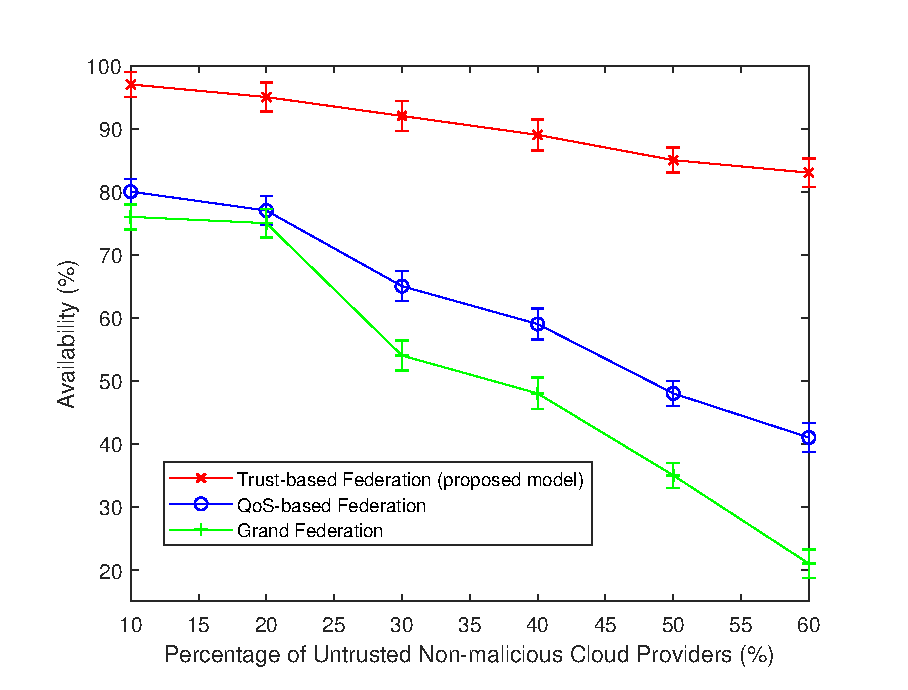
\includegraphics{availability.eps}}
\caption{availability}
\end{subfigure}
\qquad\qquad
\begin{subfigure}{\textwidth}
\centering
\scalebox{0.45}{\includegraphics{responsetime1.eps}}
\caption{response time}
\end{subfigure}
\qquad\qquad
\begin{subfigure}{\textwidth}
\centering
\scalebox{0.45}{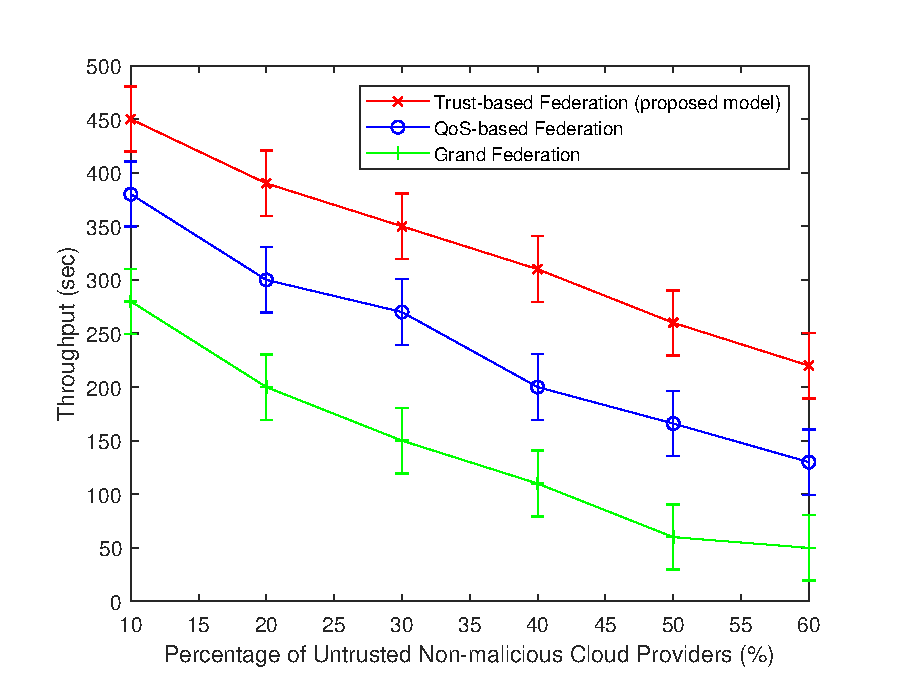
\includegraphics{throuput.eps}}
\caption{throughput}
\end{subfigure}
\qquad\qquad
\caption{Our trust-based model improves the availability, response time, and throughput compared to the grand and QoS-based federations: In the presence of untrusted non-malicious CPs}
\end{figure}


Figure 2b depicts the performance of the produced federations
in terms of response time. The response time represents
the time span between the submission and the response of
the request, which includes both the execution and the waiting
times. Figure 2b reveals that our model yields much less
response time compared to the grand and QoS-based
models in the presence of untrusted non-malicious
CPs. This is also due to the fact that our trust-based model
minimizes the percentage of untrusted non-malicious CPs
in the federation.

Figure 2c, illustrates how effective are the formed federations
in terms of throughput. Throughput describes the number
of requests that a federation can handle in a given time. In
our simulations, throughput was measured per second.
Figure 2c reveals that our trust-based model yields much
higher throughput compared to the other two models in
the presence of untrusted non-malicious CPs for the aforementioned reasons.

Next, Figures 3a, 3b, and 3c indicate the performance of our framework with respect to the number of malicious
CPs. We analyse how effective are the formed federations
in terms of availability, response time and throughput.
More specifically, Figure 3a shows the efficiency of the
formed federation in terms of availability. The figure
reveals that our model outperforms both the grand
and QoS-based models whose performance begins to
decrease largely. This is due to the fact that the proposed trust-based federation formation algorithm (Algorithm 1) compares all the possible federations
and builds preferences over them based on the federation trust criterion (Eq. 20), which in turn
minimizes the percentage of malicious CPs
in the federated CPs. In other words, it minimizes
the number of CPs that refuse to share their requested resources.

Figure 3b displays the performance of the produced federations
in terms of response time. The figure reveals that our
model yields lower response time compared to the
grand and QoS-based models in the presence of
malicious CPs. This is also due to the fact that our trust-based
model minimizes the percentage of malicious
CPs in the federation according to the preference function in Algorithm 1. Also in Figure 3c, we see the efficiency of the
formed federations in terms of throughput, which reveals
that our trust-based model yields much higher throughput
compared to the other two models in the presence of
malicious CPs.

We now carefully investigate the reasons why our model outperforms the other
studied models. More specifically, we study the percentage of malicious and untrusted non-malicious CPs that exist in the final federations. Figure 4a shows the percentage of malicious CPs that exist in the final federations structure with respect to the percentage of malicious CPs that existed in the initial federation. In other words, our goal is to study how effective is each of the compared models in avoiding the malicious CPs during federation’s formation. We exclude the grand federation approach in this study as we will end up with a single grand federation in which all CPs are members.

Figure 4a shows that the percentage of malicious CPs in the final federations keeps increasing in the QoS-based, and
our trust-based federation formation models (i.e. our model) with the increase in their percentage in the initial partition. However, our model is more resilient to that increase and is able to minimise the percentage of untrusted non-malicious CPs up to 35\% compared to the QoS-based federation approach. The reason is that our model takes into consideration the trust relationships among CPs and excludes malicious CPs during federation formation. Figure 4b depicts the efficiency of each of the compared models in avoiding the untrusted non-malicious CPs during federation’s formation. Figure 4b shows that the percentage of untrusted non-malicious CPs in the final federations also keeps increasing in the QoS-based, and our trust-based federation formation models (i.e. our model) with the increase in their percentage in the initial partition. However, our model is more resilient to that increase and is able to reduce the percentage of malicious CPs up to 27\% compared to the other models.

\begin{figure}[!ht]
\centering
\begin{subfigure}{\textwidth}
\centering
\scalebox{0.45}{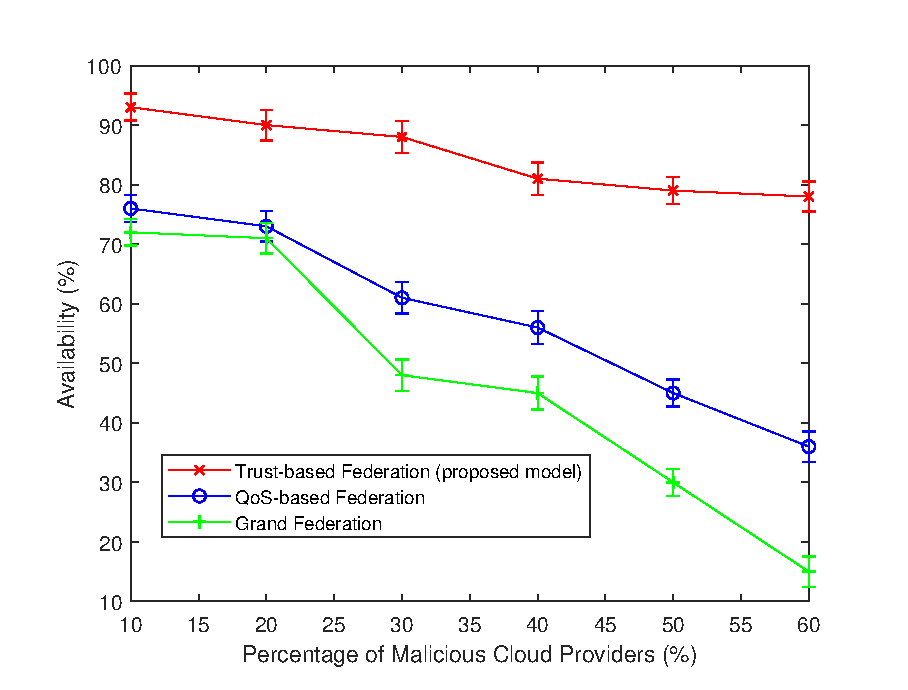
\includegraphics{Mal_availability.eps}}
\caption{availability}
\end{subfigure}
\qquad\qquad
\begin{subfigure}{\textwidth}
\centering
\scalebox{0.45}{\includegraphics{Mal_responstime.eps}}
\caption{response time}
\end{subfigure}
\qquad\qquad
\begin{subfigure}{\textwidth}
\centering
\scalebox{0.45}{\includegraphics{Mal_throughput.eps}}
\caption{throughput}
\end{subfigure}
\qquad\qquad
\caption{Our trust-based model improves the availability, response time, and throughput compared to the grand and QoS-based federations: In the presence of malicious CPs}
\end{figure}

\begin{figure}[!ht]
\centering
\begin{subfigure}{\textwidth}
\centering
\scalebox{0.45}{\includegraphics{untrusted.eps}}
\caption{Percentage of Untrusted Non-malicious Cloud Providers.}
\end{subfigure}
\qquad\qquad
\begin{subfigure}{\textwidth}
\centering
\scalebox{0.45}{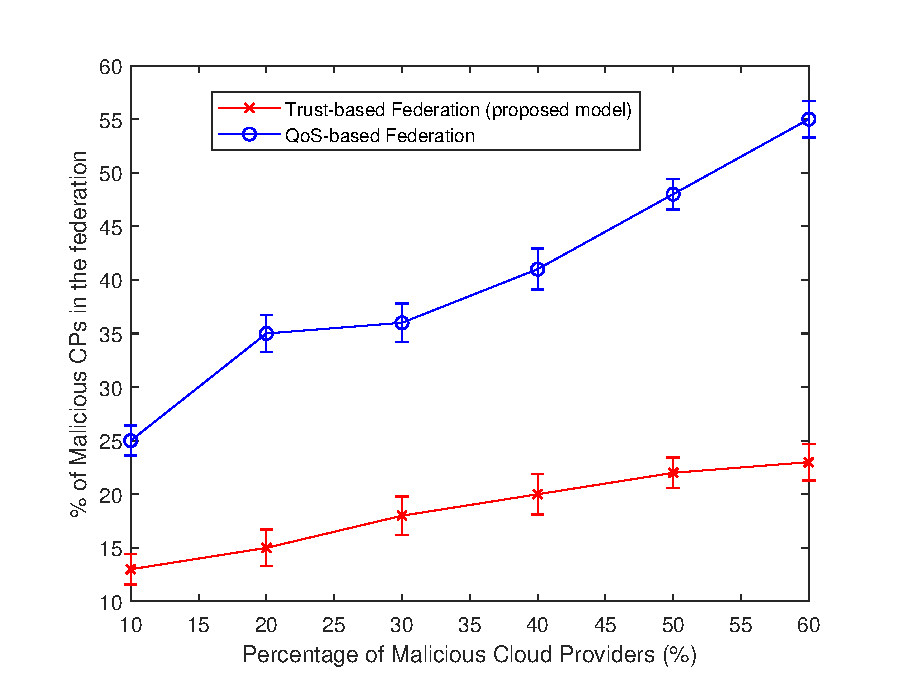
\includegraphics{mal.eps}}
\caption{Percentage of malicious Cloud Providers.}
\end{subfigure}
\centering
\qquad\qquad
\caption{Our trust-based model minimizes the number of untrusted non-malicious and malicious CPs.}
\end{figure}

%\begin{figure}[!ht]
% \scalebox{0.55}{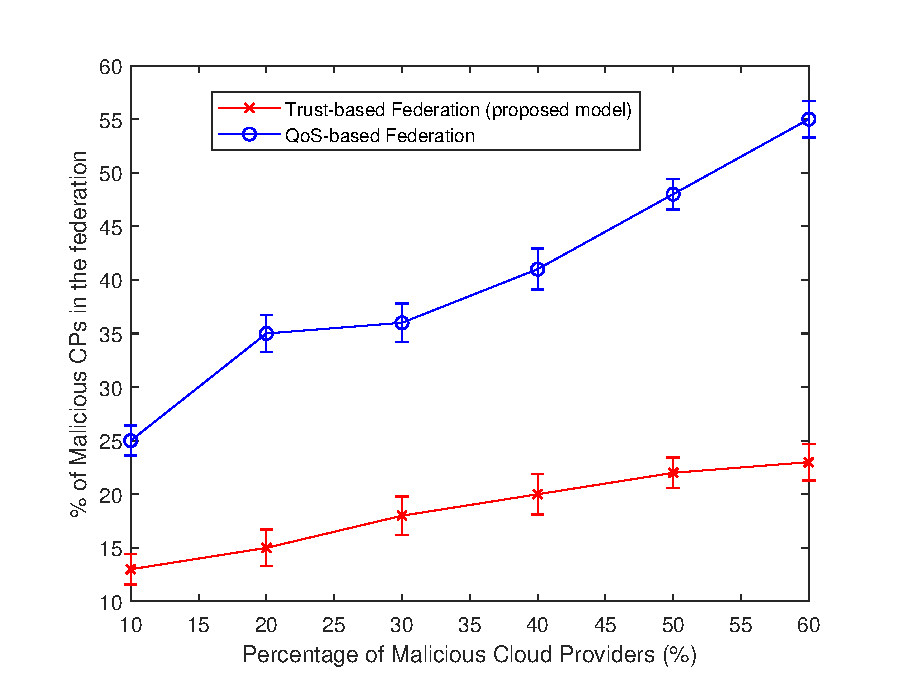
\includegraphics{mal.eps}}
% \label{fig1}
% \caption{Percentage of malicious Cloud Providers: Our trust-based model minimizes the number of malicious Cloud Providers.}
%\end{figure}

\section{Conclusion and Future Work}

In this paper, we proposed a decentralised framework that considers trustworthiness of heterogeneous CPs during
the formation of cloud computing federations. We proposed two approaches for evaluating the CPs' trust values: objective and subjective trust evaluations. In the former, the trust value is evaluated based on the history of interactions (i.e. experience) using Bayesian inference. In the latter, we used the Dempster-Shafer Theory (DST) of evidence to evaluate the trust value in the absence of previous interactions. Thereafter, we devised a federation formation algorithm, based on the coalitional game theory, that allows a set of CPs to cooperatively set up their federations in order to maximise the trust of the formed federations. We have shown that the proposed federation formation algorithm converges to a Nash-stable situation, i.e. no CP has an incentive to leave its current federation to move to another federation. Our experimental results show that the proposed federation formation algorithm minimizes the number of malicious and untrusted CPs in the federation up to 35\% compared to two state-of-the-art federation approaches. Moreover,
the performance of the formed federations in terms of availability, response time and throughput is improved.

In our future work, we will enhance our trust-based federation model to consider profit maximization during cloud federation formation.


\section*{Acknowledgments}
The financial support of the Natural Sciences and Engineering Research Council of Canada is gratefully acknowledged.

\bibliographystyle{elsarticle-num}
\bibliography{bibo}
\vspace{10 mm}
\section*{Author Biographies}
 \begin{wrapfigure}{l}{25mm}
    
\includegraphics[width=1in,height=1.25in,clip,keepaspectratio]{Adel.eps}
  \end{wrapfigure}\par
\textbf{Adel Abusitta} is a Ph.D. student in Computer Engineering at Ecole Polytechnique de Montreal, Canada. He holds a M.Sc. degree in computer science from the University of Jordan, Jordan. The main topics of his current research activities are security in Cloud Computing, network security, and authorship analysis.\par\par
\vspace{25 mm}
\begin{wrapfigure}{l}{15mm}
     \vspace{-35 mm}
    \includegraphics[width=1in,height=1.25in,clip,keepaspectratio]{Martine.eps}
  \end{wrapfigure}\par
\textbf{Martine Bellaiche} is Assistant Professor in Department of Computer and Software engineering of Ecole Polytechnique of Montreal. She received a MSc in Computer Science from University of Montreal in 1985 and the Ph.D in Telecommunications from INRS in 2007. Her research interests are in Network Security with special focus on attack, in Network Sensor Security and cloud computing security.\par
\begin{wrapfigure}{l}{25mm}
    \includegraphics[width=1in,height=1.25in,clip,keepaspectratio]{Michel.eps}
  \end{wrapfigure}\par
\textbf{Michel Dagenais} is professor at Ecole Polytechnique de Montreal in the department of Computer and Software Engineering. He authored or co-authored over one hundred scientific publications, as well as numerous free documents and free software packages in the fields of operating systems, distributed systems and multicore systems, in particular in the area of tracing and monitoring Linux systems for performance analysis. Most of his research projects are in collaboration with industry and generate free software tools among the outcomes. The Linux Trace Toolkit next generation, developed under his supervision, is now used throughout the world and is part of several specialized and general purpose Linux distributions.
\end{document}

\end{document} 